\begin{center}
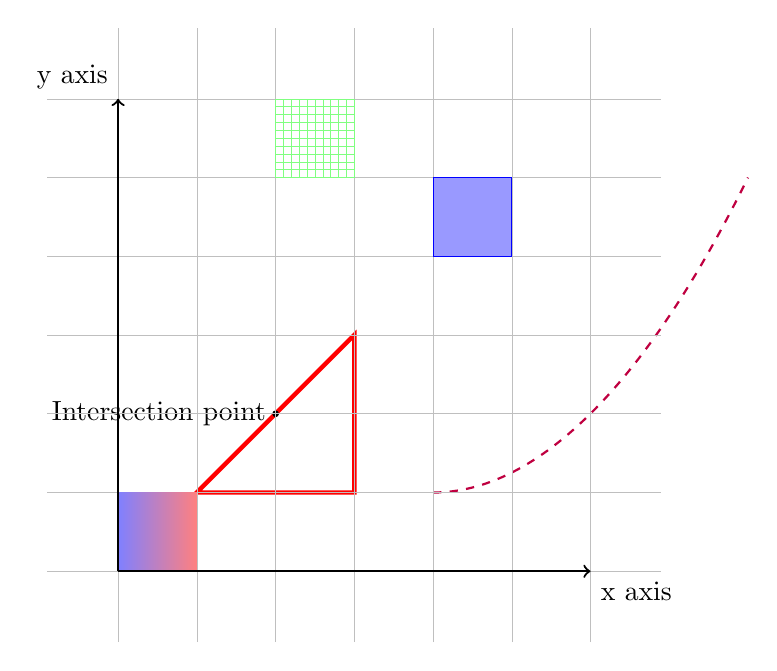
\begin{tikzpicture}

\draw[red, ultra thick] (0,0) -- (2,0) -- (2,2) -- cycle;
\filldraw[black] (1,1) circle (1pt) node[anchor=east] {Intersection point};
\draw[purple, dashed, thick] (3,0) parabola (7,4);
\draw[step = 1cm, gray!50, very thin] (-1.9,-1.9) grid (5.9,5.9);
\draw[step = 0.1cm, green!50, very thin] (1,4) grid (2,5);
\fill[blue!40!white, draw=blue] (3,3) rectangle (4,4);
\shade[left color=blue!50, right color=red!50] (0,0) rectangle (-1,-1);

\draw[thick, ->] (-1,-1) -- (5,-1) node[anchor=north west] {x axis};
\draw[thick, ->] (-1,-1) -- (-1,5) node[anchor=south east] {y axis};



\end{tikzpicture}   
\end{center}